%------------------------------------------------------------
%------------    Estrutura do texto   -----------------------         


\usepackage[small,bf]{caption} % captions e legends fonte reduzida

\usepackage{multirow} % Tabela mesclar linhas
\usepackage{multicol} % Tabela mesclar colunas

% Pacotes Básicos:
\usepackage{lmodern}			    % Usa a fonte Latin Modern			
\usepackage[T1]{fontenc}		  % Selecao de codigos de fonte.
\usepackage[utf8]{inputenc}		% Codificacao do documento (conversão automática dos acentos)
\usepackage{lastpage}			    % Usado pela Ficha catalográfica
\usepackage{indentfirst}		  % Indenta o primeiro parágrafo de cada seção.
\usepackage{color}				    % Controle das cores
\usepackage{graphicx}			    % Inclusão de gráficos
\usepackage{microtype} 		  	% para melhorias de justificação

% Pacotes Extras:

\usepackage{amsmath,amsthm}   %Símbolos Matemáticos
\usepackage{indentfirst} % Indenta primeiro parágrafo 
\usepackage[portuguese, ruled, linesnumbered,commentsnumbered, algo2e, vlined, lined, boxed, algochapter]{algorithm2e} % Algoritmos 
\usepackage{hyperref}
\usepackage[brazilian,hyperpageref]{backref}	 % Paginas com as citações na bibliograficas
\usepackage[alf]{abntex2cite}	% Citações padrão ABNT
\usepackage{etoolbox}
%\usepackage[num]{abntex2cite}  % Citações numéricas

%inclusao PDF
\usepackage{pdfpages}

% Defininfo Cores:
\definecolor{blue}{RGB}{25,25,112}

\makeatletter % informações do PDF
\hypersetup{ % pagebackref=true,
	pdftitle={\@title}, 
	pdfauthor={\@author},
    pdfsubject={\imprimirpreambulo},
	pdfcreator={LaTeX with abnTeX2},
	pdfkeywords={abnt}{latex}{abntex}{abntex2}{trabalho acadêmico}, 
	colorlinks=true,     % false: boxed links; true: colored links
    linkcolor=blue,          	% color of internal links
    citecolor=blue,        		% color of links to bibliography
    filecolor=magenta,      	% color of file links
    urlcolor=blue,
	bookmarksdepth=4 }
\makeatother
 

% -------------------------------------------- 
% Espaçamentos entre linhas e parágrafos 
\setlength{\parindent}{1.3cm} % O tamanho do parágrafo

% Controle do espaçamento entre um parágrafo e outro:
\setlength{\parskip}{0.2cm}  % tente também \onelineskip

% Definição de ambientes matemáticos em português 
\newtheorem{teorema}{Teorema}[chapter]
\newtheorem{axioma}{Axioma}[chapter]
\newtheorem{corolario}{Corolário}[chapter]
\newtheorem{lema}{Lema}[chapter]
\newtheorem{proposicao}{Proposição}[chapter]
\newtheorem{definicao}{Definição}[chapter]
\newtheorem{exemplo}{Exemplo}[chapter]
\newtheorem{observacao}{Observação}[chapter]

% Novos Comandos
\usepackage{tgtermes}
\renewcommand{\ABNTEXchapterfont}{\rmfamily\bfseries}

% Variáveis adicionais
\providecommand{\imprimirautorcite}{}
\newcommand{\autorcite}[1]{\renewcommand{\imprimirautorcite}{#1}} 
\providecommand{\imprimirsigla}{}
\newcommand{\sigla}[1]{\renewcommand{\imprimirsigla}{#1}}
\providecommand{\imprimiruf}{}
\newcommand{\uf}[1]{\renewcommand{\imprimiruf}{#1}}
\providecommand{\imprimircurso}{}
\newcommand{\curso}[1]{\renewcommand{\imprimircurso}{#1}}
\providecommand{\imprimirinstituto}{}
\newcommand{\instituto}[1]{\renewcommand{\imprimirinstituto}{#1}}
\providecommand{\imprimirdepartamento}{}
\newcommand{\departamento}[1]{\renewcommand{\imprimirdepartamento}{#1}}
\providecommand{\imprimirano}{}
\newcommand{\ano}[1]{\renewcommand{\imprimirano}{#1}}
\providecommand{\imprimirgrau}{}
\newcommand{\grau}[1]{\renewcommand{\imprimirgrau}{#1}}
\providecommand{\imprimirexaminadorum}{}
\newcommand{\examinadorum}[1]{
    \renewcommand{\imprimirexaminadorum}{#1}}
\providecommand{\imprimirexaminadordois}{}
\newcommand{\examinadordois}[1]{
    \renewcommand{\imprimirexaminadordois}{#1}}
\providecommand{\imprimirexaminadortres}{}
\newcommand{\examinadortres}[1]{
    \renewcommand{\imprimirexaminadortres}{#1}}
\providecommand{\imprimirexaminadorquatro}{}
\newcommand{\examinadorquatro}[1]{
    \renewcommand{\imprimirexaminadorquatro}{#1}}
\providecommand{\imprimirttorientador}{}
\newcommand{\ttorientador}[1]{
    \renewcommand{\imprimirttorientador}{#1}} 
\providecommand{\imprimirttcoorientador}{}
\newcommand{\ttcoorientador}[1]{
    \renewcommand{\imprimirttcoorientador}{#1}}
\providecommand{\imprimirttexaminadorum}{}
\newcommand{\ttexaminadorum}[1]{
    \renewcommand{\imprimirttexaminadorum}{#1}}
\providecommand{\imprimirttexaminadordois}{}
\newcommand{\ttexaminadordois}[1]{\renewcommand{
        \imprimirttexaminadordois}{#1}}
\providecommand{\imprimirttexaminadortres}{}
\newcommand{\ttexaminadortres}[1]{
    \renewcommand{\imprimirttexaminadortres}{#1}}
\providecommand{\imprimirttexaminadorquatro}{}
\newcommand{\ttexaminadorquatro}[1]{
    \renewcommand{\imprimirttexaminadorquatro}{#1}}

%----------------------------------------------------
\renewcommand{\imprimircapa}{  % Capa 
\begin{capa}

\hspace{-3cm}
\begin{tabular}{c c c}
    \centering
    
\includegraphics[scale=0.45]{figuras/profept_clean.jpg} &
    \large \imprimirinstituicao  &
    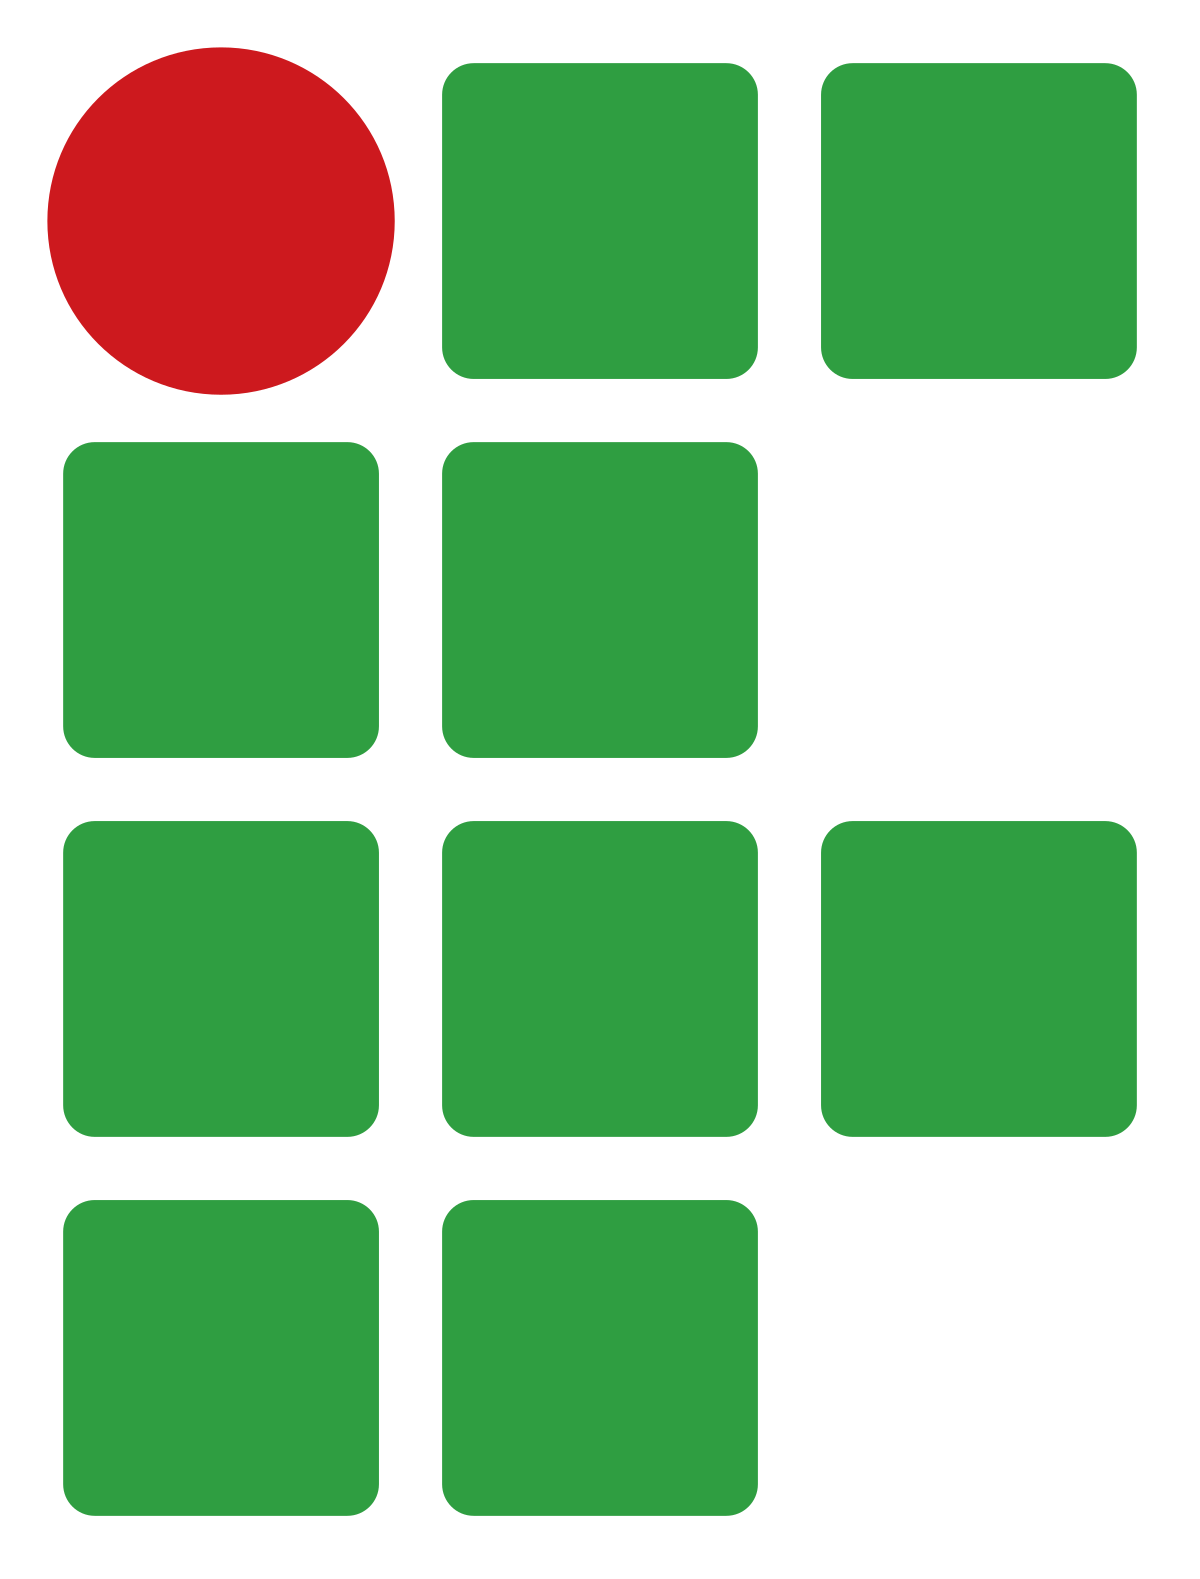
\includegraphics[scale=0.04]{figuras/ifap_clean.png}\\
    & \large \imprimirinstituto & \\
    & \large \imprimirdepartamento & \\
    
    
\end{tabular}






%\hspace{-1cm} \begin{minipage}[b]{0.19\linewidth}
%              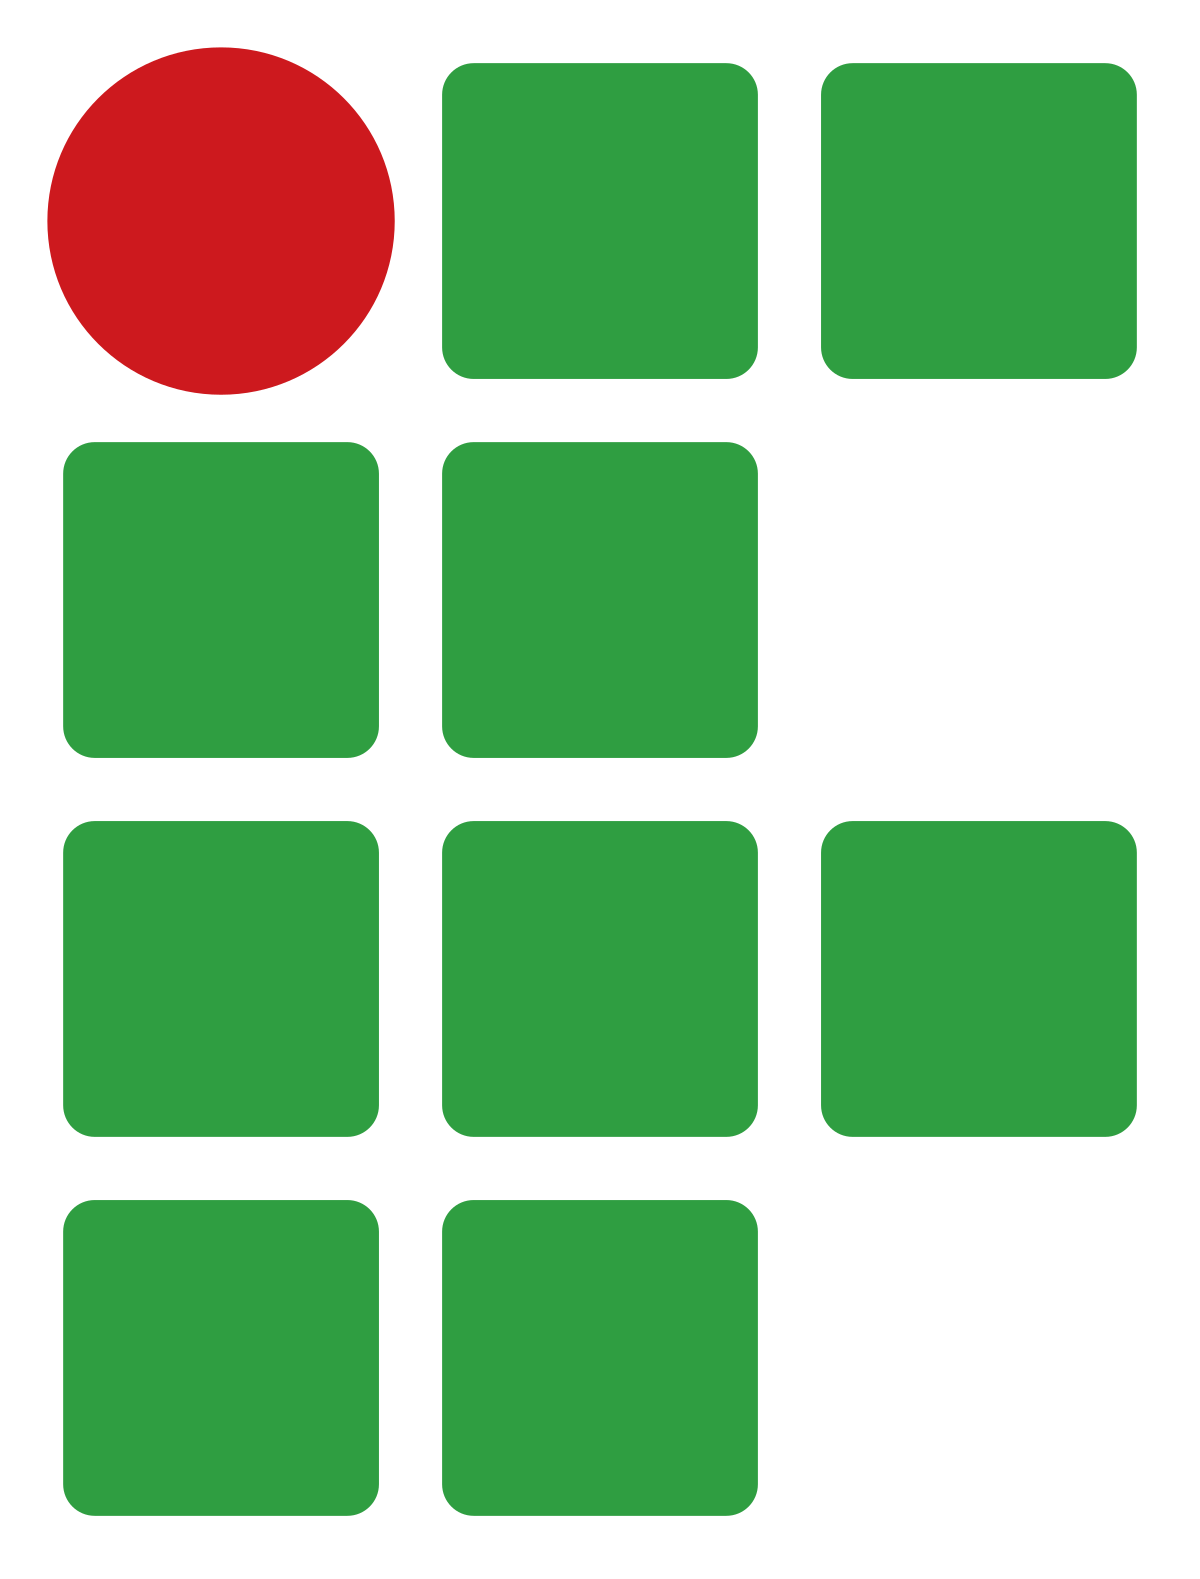
\includegraphics[scale=0.04]{figuras/ifap_clean.png}
%              \end{minipage}
%\hspace{-1cm} \begin{minipage}[b]{0.68\linewidth}
%              \begin{center}{\large
%              Ministério da Educação \\
%              \imprimirinstituicao \\
%              \imprimirinstituto \\
%              \imprimirdepartamento }\end{center}
%              \end{minipage} 
%\begin{minipage}[b]{0.15\linewidth}
%
\includegraphics[scale=0.45]{figuras/profept_clean.jpg}
%\end{minipage}


\vfill
        \begin{center}
        {\textsc{\huge \textbf{\imprimirtitulo}}}  \\
        
       
				\vspace{2cm}
				{\textsc {\large \imprimirautor}} 	
				\vfill
        {\large{\imprimirlocal~ - \imprimiruf \\ \imprimirano  }}
        \end{center}
\end{capa}   } % Capa

%----------------------------------------------------
\renewcommand{\imprimirfolhaderosto}{% folha de rosto
    \begin{center}
    {\textsc {\large \imprimirautor}}  \\
		\vfill
		{\textsc{\Huge \textbf{\imprimirtitulo}}}
    \end{center}
    \vfill 
    \begin{flushright} 
    \parbox{0.6\linewidth}{
		\imprimirtipotrabalho~ apresentada ao curso de \imprimircurso~ do \imprimirinstituicao~ como parte dos
		requisitos necessários para a obtenção do grau em \imprimirgrau. \\
		\vfill
		\textbf{\imprimirorientadorRotulo}~\imprimirorientador \\
		\vfill 
		\textbf{\imprimircoorientadorRotulo}~\imprimircoorientador}
   \end{flushright} 
   
	 \vfill
   \begin{center}
   {\large{\imprimirlocal~ - \imprimiruf \\ \imprimirdata}}
   \end{center} }  % folha de rosto

%----------------------------------------------------


